\documentclass[12pt, a4paper, showtrims]{article}
\usepackage{geometry}
\usepackage{ragged2e}
\usepackage{graphicx}
\usepackage{wrapfig}
\usepackage{csvsimple}




\graphicspath{ {./images/} }
\geometry{a4paper, top=2cm, bottom=2cm,
          hmargin=2.3cm,  includehead, includefoot}




\begin{document}

\title{Emek Ekonomisi Ödev-1 Çözümleri}
\author{Yasemin Hayırlı}
\date{14 Aralık 2020}
\maketitle

\section{a}
\subparagraph*{Kukla Değişkenler} 
\begin{justify}
Kukla değişkenler, regresyon analizinde bağımsız değişkenlerin
kategorik olarak gösterimini sağlar ve n adet kukla değişkenden bir tanesi 
referans alınarak kukla değişkenler arasında karşılaştırma yapılır. 
    
Angrist ve Krueger(1991) yaptıkları çalışmada doğum çeyreklerini kukla 
değişken olarak kullanmışlardır. Doğum çeyreklerini 4 adet tanımladıklarından 
dolayı n-1 tane yani 3 adet kukla değişken oluşturulmalıdır.

Aşağıdaki regresyon denklemi doğum çeyreklerinin eğitim seviyeleri üzerindeki etkisini
tahmin etmektedir. Ancak denklem trendden arındırılmamıştır.

\[ E_{icj} = \alpha + \sum_{j}^{3}\beta_jQ_{icj} + \epsilon_{icj}  \]
\begin{figure}[h]
    \caption{Doğum Çeyreklerinin Eğitim Üzerindeki Etkisi}
    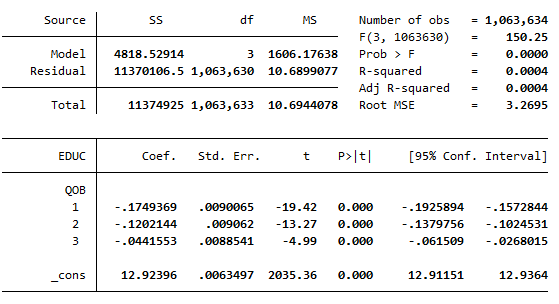
\includegraphics[width=14cm, height=5cm]{dummy_var_1.png}
    \centering
\end{figure}

\begin{table}[h!]
    \centering
    \caption{Table to test captions and labels}
    \begin{tabular}{||c c c c||} 
     \hline
     Col1 & Col2 & Col2 & Col3 \\ [0.5ex] 
     \hline\hline
     1 & 6 & 87837 & 787 \\ 
     2 & 7 & 78 & 5415 \\
     3 & 545 & 778 & 7507 \\
     4 & 545 & 18744 & 7560 \\
     5 & 88 & 788 & 6344 \\ [1ex] 
     \hline
    \end{tabular}
    
    \label{table:1}
    \end{table}




\begin{wrapfigure}{h}{0.25\textwidth}
    \centering
    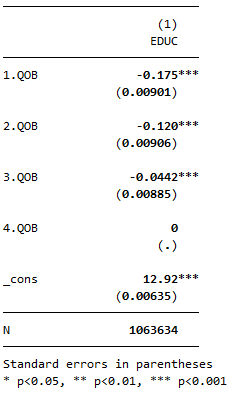
\includegraphics[width=0.25\textwidth]{dummy_var_1_2.png}
\end{wrapfigure}

     
\end{justify}

\end{document}